\documentclass[11pt,a4paper]{article}

\usepackage[T1]{fontenc}
\usepackage[utf8]{inputenc}
\usepackage{lmodern}
\usepackage[margin=2.4cm]{geometry}
\usepackage{amsmath,amssymb,bm}
\usepackage{booktabs,array,tabularx,multirow}
\usepackage{graphicx}
\usepackage{enumitem}
\usepackage{xcolor}
\usepackage{tikz}
\usetikzlibrary{arrows.meta,decorations.pathreplacing,calc,patterns}
\usepackage{xr-hyper}
\usepackage[colorlinks=true,linkcolor=teal!70!black,citecolor=teal!70!black,urlcolor=teal!70!black]{hyperref}
\usepackage{caption}
\captionsetup{font=small,labelfont=bf}
% Cross-references to the supplementary file (labels prefixed S-).
\externaldocument[S-]{paper2_supplement}

\setlength{\parskip}{0.4em}
\setlength{\parindent}{0pt}
\newcommand{\nj}{\textsc{nj}}
\newcommand{\nh}{\textsc{nh}}
\newcommand{\thead}{\tau_{\mathrm{cross}}}
\newcommand{\tcross}{\tau_{\mathrm{cross}}}
\newcommand{\tpp}{\tau_{\mathrm{pp}}}
\newcommand{\tv}{\tau_{v}}
\newcommand{\lv}{\ell_{v}}
\newcommand{\vb}{v_{\mathrm{belt}}}
\newcommand{\supsec}[1]{Supplementary Section~\ref{S-#1}}

\title{\textbf{How Far Must the Camera See?}\\[0.3em]
\large The value of upstream visibility and pre-positioning in a shared-head conveyor cell,
across geometries and operating conditions}
\author{laser-conveyor-optimization\\\small\url{https://github.com/juanlopez-gif/laser-conveyor-optimization}}
\date{November 2026 --- short version of draft 1.6 (version 0.7.42)}

\begin{document}
\maketitle

\begin{abstract}
A single XY laser head serves three parallel conveyors that stop while a part is
processed or blocked; a camera may see the belts upstream of the head's working zone. We
ask how far upstream it must see, and whether its value comes from seeing earlier or from
acting earlier. Three paired simulation studies answer it: a reference cell, a geometry
bench at 3~cm/s (56 distinct cells; three analyses: two tie-breaks, then fresh
realizations) and a belt-speed bench. At 5~cm/s, with a dispatching rule and its observable tie-break (60 reserved
realizations, seeds 10000--10059), a 10~cm view
cost less than a 0.5~s-per-part margin fixed beforehand against the full 50~cm view in
both geometries with the fast along-belt head axis (upper 95\,\% bounds 0.33 and 0.23~s
per part); neither slow-axis geometry met the full-view benefit criterion. In the
reference cell (seeds 7000--7029; rule with its arrival-time tie-break), acting on the view
reduced the penalized flow time by 7.4\,\% at the nominal load for the rule and a learned
policy (2.7--4.3\,\% with bursts or a slow head);
seeing alone changed little. Where pre-positioning pays at 3~cm/s, 3.33~s of anticipation
instead of 10~s cost the rule a median of 0.05, 0.04 and 0.09~s per part in the three analyses
(largest observed estimates 0.44, 0.44 and 0.47, not bounds for the family).
Retaining 90\,\% of the gain was certified before 10~s in 17 of 18 cells with the
arrival-time tie-break, but in 3 of 19 (same realizations) and 1 of 14 (fresh realizations)
with the observable one. For this cell family at
3~cm/s the camera can be specified in seconds of belt motion; transfer across belt speeds remains
open.
\end{abstract}

%====================================================================
\section{Introduction}
%====================================================================
Cells in which one shared actuator serves several moving streams are common in sorting,
packaging and marking lines \cite{S01_Mattone2000,S02_Han2020,S03_Nielsen2023,S04_Schettini2023}.
The actuator reaches a bounded window of each stream; what the controller can decide
depends on what it sees. Instrumentation (which stretch of the belts a camera covers) and
capability (whether the head may move towards a part before it is reachable) are design
choices that are usually fixed before the scheduling policy is written. The value of
seeing further has been measured for an operator's inspection range \cite{Nawijn1981},
for item-count lookahead in robot sorting \cite{Li2026} and for the length of an upstream
buffer combined with the reach of several packing arms \cite{Ladefoged2026}; separating
the value of the view from the value of the action it enables, for a head shared by belts
that stop, has not been measured to our knowledge.

The cell (Section~\ref{sec:cell}) has one Cartesian laser head over three parallel
conveyors. A part can be processed only inside the laser zone; while it is processed its
conveyor stops, and an unprocessed part that reaches the end of the zone stops its
conveyor until the head serves it (blocking). The controller's objective is the mean flow
time plus a penalty for blocking. An overhead camera sees the laser zone and, upstream of
it, a stretch of the entry zone; the coverage corresponds to $\tv$ seconds of
uninterrupted belt motion before a part becomes reachable, the camera's
\emph{anticipation}. Two things change when the camera sees further. The controller
\emph{sees} parts earlier, so that it may choose better among the parts already in the
zone; and, if the cell allows it, it may \emph{act} earlier: send the idle head to the
entry point of a belt on which a part is approaching. The pilot of this work took the
head's travel time across the conveyors, $\tcross$, as the reference for sizing the
coverage; the geometry bench was designed to test that reference.

\textbf{Contributions.} All studies are paired simulations with protocols frozen before
the run; \nj\ is the dispatching rule used as primary controller.
\begin{enumerate}[nosep]
\item \emph{What transfers to a faster belt} (Section~\ref{sec:belt}). At a belt speed of
  5~cm/s, in the two tested geometries with the fast along-belt head axis ($v_x=10$~cm/s;
  $d/v_y=12/10$ and $6/15$), a 10~cm view met the loss margin of 0.5~s per part fixed
  beforehand against the full 50~cm view (\nj\ with the observable tie-break; belt-speed
  bench, 60 reserved realizations, seeds 10000--10059); neither slow-axis geometry met the full-view benefit
  criterion at 5~cm/s; the conservative 90\,\% retention criterion was first certified only
  at 25 and 50~cm in the fast-axis cells; whether the coverage scales in seconds or in
  centimetres remains open.
\item \emph{Seeing against acting} (Section~\ref{sec:reference}). In a reference cell
  (eight regimes; seeds 7000--7029, shared with the companion paper), widening the view
  with the same actions produced small effects, while acting on it reduced the penalized
  flow time by 7.4\,\% at the nominal regime for both the rule and a learned policy, and by
  2.7--4.3\,\% with bursts or a slow head.
\item \emph{The cost of a shorter view at 3~cm/s} (Section~\ref{sec:cost}). In the cells
  of a 56-cell geometry bench where pre-positioning pays, 3.33~s of anticipation instead of
  10~s cost a median of 0.05, 0.04 and 0.09~s per part in three analyses (arrival-time
  tie-break and observable tie-break on seeds 9000--9059; observable tie-break on fresh
  seeds 43700--43759); the largest estimates, 0.44, 0.44 and 0.47~s per part, are observed
  values with individual intervals, not bounds for the family.
\item \emph{Certified 90\,\% retention} (Section~\ref{sec:retention}). Retaining 90\,\% of
  the gain was certified before 10~s in 17 of 18 cells with the arrival-time tie-break, but
  in 3 of 19 and 1 of 14 with the observable one; which cells pass the benefit screen is not
  stable across realizations.
\item \emph{Design factors} (Section~\ref{sec:vx}). The along-belt head speed $v_x$ is a
  first-order factor; the crossing time $\tcross$ is the poorest predictor of the required
  anticipation, and no predictor probed supports extrapolation beyond the cells tested.
\end{enumerate}
The companion paper (Paper~1) presents the learned policy used here; this paper uses it
only as a secondary controller and does not depend on its training. Material moved out of
this version (per-cell tables, all bench curves, predictors, mechanism, entry length,
checks, pilot and robustness analyses) is in the Supplementary Material, cited as
Supplementary Sections~\ref{S-sup:related}--\ref{S-sup:discussion}.

%====================================================================
\section{Related work}\label{sec:related}
%====================================================================
Five strands of work touch the cell studied here; the full discussion is in
\supsec{sup:related}.

\textbf{Lookahead and upstream information.} Three studies ask how much a controller gains
from seeing further ahead, each in a different setting from ours. At a conveyor-serviced
station with Poisson arrivals, an operator inspects a range of the belt measured in time
units; units that pass are lost and the belt never stops \cite{Nawijn1981}. A robot arm
that takes the foremost item of one of several infeed queues, with the next $L$ items of
each queue identified, is within about 1\,\% of its full-information optimum on average
already at $L=1$ when it votes over sampled completions of the hidden queues
\cite{Li2026}: lookahead is counted in item identities, and the robot cannot act on an
item before it is at the pick point. In robotic food packing, a buffer belt ahead of four
arms with exclusive zones sets how early item weights are known; a longer buffer reduces
the overfill with diminishing returns and its value interacts with the reach given to each
arm \cite{Ladefoged2026}. Their formulation includes the time an arm needs to intercept an
item, pack it and reach the next one, but the reported simulations assume instantaneous
movements and tray swaps, so moving an arm ahead of an item is not studied; the belts run
at constant speed and never stop, and the effects are fitted by regression on
dimensionless parameters. Our study varies the physical length the camera covers and,
separately, the permission to send a shared head towards a part before it is reachable,
on belts that stop, and estimates both effects on paired realizations with criteria fixed
before the run. The horizon of a look-ahead controller \cite{Righettini2025} truncates
simulated futures; the anticipation measured here is what the camera physically observes
now.

\textbf{Picking and sorting from moving conveyors.} Single-arm sequencing by dynamic
programming \cite{S02_Han2020}, sorting on a moving belt \cite{S01_Mattone2000},
value-aware sorting with availability windows \cite{S05_Kokkalis2026}, multi-arm batching
in which a longer buffer zone improves the objective but raises the computation beyond its
budget \cite{S03_Nielsen2023}, and robot scheduling with cameras that see items 5--10~s
ahead \cite{S04_Schettini2023} all have belts that never stop because of the processing,
and unserved items leave the system. In our cell processing stops the part's belt and an
unprocessed part blocks it, so the trajectories of the remaining parts depend on the
schedule, and the visibility horizon is measured rather than fixed. Stops caused by
unfinished work are classical in mixed-model assembly lines \cite{Xiaobo2000,Tamura2011},
where the launch sequence is fixed offline and nothing is sensed.

\textbf{Interception of moving targets.} Moving-target travelling salesman models
\cite{S06_Helvig2003,S07_Stieber2022,S08_Philip2024} give exact offline models of an agent
intercepting targets with exogenous, constant velocities; our cell uses the same
interception geometry with endogenous motion, since a belt's odometer stops while its part
is processed or blocked.

\textbf{Blocking in conveyor systems.} Blocking as a schedule-dependent loss appears in
packaging machines whose devices obstruct each other \cite{S10_Briskorn2025} and in a food
warehouse whose full crane buffers stop upstream conveyors \cite{S11_SalviaHornos2026}.
Our objective charges both the blocking events and their duration, inside the dispatching
problem.

\textbf{Learned dispatching.} The secondary controller belongs to the family of
dispatching policies trained from search or from expert schedules
\cite{M02_Bertsekas1997,S19_Zhang2020,S21_Sun2023,S20_VanRemmerden2025,M04_Huang2022,S18_Wei2024}
and of learned control of conveyor-fed robotic cells
\cite{S15_Zisgen2025,S16_Drijver2023,S17_Drakaki2017,S12_Wang2004,S13_Li2020}. Here it
matters only that it uses every observable part, so that it can turn a wider view into
different decisions, which the dispatching rule with the arrival-time tie-break cannot.

What these works leave open, and this paper measures, is how the value of the sensing
reach depends on what the controller may do with it, and how that value moves with the
geometry, the load and the belt speed of the cell, on paired realizations.

%====================================================================
\section{The cell and its information model}\label{sec:cell}
%====================================================================

\subsection{Geometry and dynamics}
Figure~\ref{fig:cell} shows the cell. Parts travel in the $+x$ direction on $N=3$
conveyors at $y_k=(k-1)\,d$, $d$ the belt spacing, at a common belt speed $\vb$. The belt
has an entry zone $[0,a)$ that the head cannot reach, a laser zone $[a,b]$ of 35~cm, and
an exit zone of 10~cm. The head moves in the rectangle $[a,b]\times[0,2d]$ with
simultaneous axes at speeds $v_x$ and $v_y$, so that the travel between two points takes
$\max(\Delta x/v_x,\Delta y/v_y)$. Processing a part takes a constant $p$ seconds, during
which the part's conveyor stops. A part that reaches $b$ unprocessed stops its conveyor
until the head serves it; every such event is a \emph{blocking} event. The \emph{reference
cell} has $d=12$~cm, an entry zone of 10~cm, $\vb=3$~cm/s, $v_x=v_y=10$~cm/s, $p=2.5$~s
and mean inter-arrival times of 10, 12 and 14~s on the three belts (processing load
$\rho_p=0.64$); its heavy variant has $\vb=5$~cm/s, $v_x=v_y=5$~cm/s, $p=3$~s and
inter-arrivals of 8, 10 and 12~s ($\rho_p=0.93$, overloaded once the head's travel is
counted). The geometry bench varies $d$, $v_y$, $v_x$ and the arrival rates and lengthens
the entry zone to 35~cm; the belt-speed bench adds $\vb=5$~cm/s with a 50~cm entry. The
formal model is given in the project's formulation document.

\begin{figure}[t]
\centering
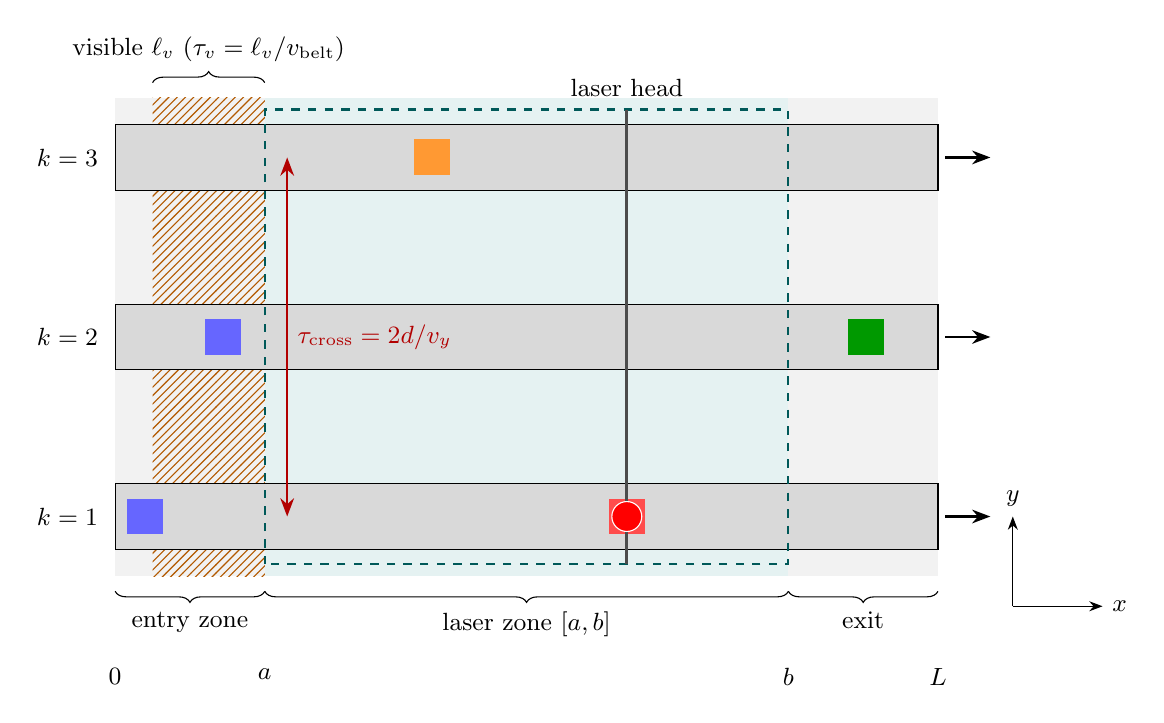
\begin{tikzpicture}[x=0.19cm,y=0.19cm,>=Stealth]
  \fill[gray!10] (0,-4) rectangle (10,28);
  \fill[teal!10] (10,-4) rectangle (45,28);
  \fill[gray!10] (45,-4) rectangle (55,28);
  \fill[pattern=north east lines,pattern color=orange!70!black] (2.5,-4) rectangle (10,28);
  \foreach \y/\n in {0/1,12/2,24/3}{
    \draw[fill=gray!30] (0,\y-2.2) rectangle (55,\y+2.2);
    \node[left] at (-0.5,\y) {\small $k=\n$};
    \draw[->,thick] (55.5,\y) -- (58.5,\y);
  }
  \draw[teal!70!black,dashed,thick] (10,-3.2) rectangle (45,27.2);
  \fill[blue!60] (0.8,-1.2) rectangle (3.2,1.2);
  \fill[blue!60] (6,10.8) rectangle (8.4,13.2);
  \fill[orange!80] (20,22.8) rectangle (22.4,25.2);
  \fill[red!70] (33,-1.2) rectangle (35.4,1.2);
  \fill[green!60!black] (49,10.8) rectangle (51.4,13.2);
  \draw[very thick,gray!60!black] (34.2,-3.2) -- (34.2,27.2);
  \draw[fill=red,draw=white] (34.2,0) circle (1.0);
  \node[above] at (34.2,27.4) {\small laser head};
  \draw[<->,thick,red!70!black] (11.5,0) -- (11.5,24) node[midway,right] {\small $\tcross=2d/v_y$};
  \draw[decorate,decoration={brace,mirror,amplitude=4pt}] (0,-5) -- (10,-5)
       node[midway,below=4pt] {\small entry zone};
  \draw[decorate,decoration={brace,amplitude=4pt}] (2.5,29) -- (10,29)
       node[midway,above=4pt] {\small visible $\lv$ ($\tv=\lv/\vb$)};
  \draw[decorate,decoration={brace,mirror,amplitude=4pt}] (10,-5) -- (45,-5)
       node[midway,below=4pt] {\small laser zone $[a,b]$};
  \draw[decorate,decoration={brace,mirror,amplitude=4pt}] (45,-5) -- (55,-5)
       node[midway,below=4pt] {\small exit};
  \node[below] at (0,-9.5) {\small $0$};
  \node[below] at (10,-9.5) {\small $a$};
  \node[below] at (45,-9.5) {\small $b$};
  \node[below] at (55,-9.5) {\small $L$};
  \draw[->] (60,-6) -- (66,-6) node[right] {\small $x$};
  \draw[->] (60,-6) -- (60,0) node[above] {\small $y$};
\end{tikzpicture}
\caption{Cell layout (top view, reference cell). Parts travel in $+x$; the head reaches
$[a,b]\times[0,2d]$. The camera sees the laser zone and the hatched stretch $[a-\lv,a)$
of the entry zone: the coverage corresponds to $\tv=\lv/\vb$ seconds of uninterrupted
belt motion before a part becomes reachable. The part on belt~1 is upstream of the visible stretch and is not seen.
$\tcross$ is the head's travel time across the conveyors.}
\label{fig:cell}
\end{figure}

\subsection{Objective}
An episode generates arrivals for 300~s and then runs until every part has left. The
objective is the \emph{penalized flow time}
\begin{equation}
J=\frac{1}{n}\sum_{j=1}^{n}(C_j-r_j)+\frac{\lambda_N N_B+\lambda_T T_B}{n},
\end{equation}
the mean flow time from arrival $r_j$ to completion $C_j$ plus a penalty for the $N_B$
blocking events and the $T_B$ conveyor-seconds stopped by blocking, with $\lambda_N=10$~s
per event and $\lambda_T=1$~s per conveyor-second. The weights are placeholders in
equivalent seconds; the economic translation is left for a later version
(Section~\ref{sec:limits}). Every gain reported below is a difference of $J$ between two
configurations on the same realization; in the geometry bench it is given in seconds per
part, and it turns out to be 82--96\,\% flow time. That share does not make threshold
decisions insensitive to the weights: with the unpenalized flow time instead of $J$, the
benefit criterion of the geometry bench (Section~\ref{sec:bench}) would pass 15 cells
instead of 18 (a sensitivity computed after the run; the penalty terms decide whether the
three cells lost reach the threshold, \supsec{sup:weights}).

\subsection{Information model and pre-positioning}
A policy may use only what the cell observes. At a dispatch event (the head is free and at
least one candidate exists) the controller knows the time, the head's position and state,
the state of every belt, and, for every \emph{observable} part, its belt, position,
processing time and the instant from which it has been observed. Three observation levels
are compared: \texttt{zone}, parts inside the laser zone only (a cell without camera);
\texttt{belts}, the above plus the parts in the visible stretch $[a-\lv,a)$ of the entry
zone ($\lv=0$ coincides with \texttt{zone}); and \texttt{full}, the above with the whole
entry zone plus the parts waiting upstream of the belt entry, which the real camera cannot
see (an upper bound on the information available, not on the value a fixed controller
realizes from it). Under \texttt{belts} a part upstream of the visible stretch is unknown
to the controller: it produces no observation, it is not a candidate, and its earlier
history leaves no trace once it appears. The controller knows the mean arrival rates and
the arrival horizon, never the future arrival instants.

The head's \emph{pre-positioning} option decides what it may do with a visible part that
is still in the entry zone. With \texttt{none} the candidates are the parts already in
the laser zone; with \texttt{when\_idle}, if no part is in the zone, the head may be sent
towards a visible entry-zone part: it moves to the point $(a,y_k)$ and waits there, and
the commitment is revoked (at no cost) the moment another part is ready in the zone while
the target is still in the entry zone, so that the policy decides again; if the target
itself enters the zone, alone or together with other parts, the commitment stands.
Physically, \texttt{when\_idle} needs the camera to cover the entry zone and the head to be
able to move to a point and wait; it is the design mode of the cell. The reference-cell
treatments combine the two options:
\begin{center}
\small
\begin{tabularx}{\linewidth}{@{}l l l X@{}}
\toprule
treatment & observation & pre-positioning & what it measures\\
\midrule
A & \texttt{zone} & \texttt{none} & no camera: local visibility, local actions\\
B & \texttt{belts}, $\lv=10$ & \texttt{none} & the camera: upstream visibility, the same actions\\
C & \texttt{belts}, $\lv=10$ & \texttt{when\_idle} & the camera and the action it enables\\
D & \texttt{full} & \texttt{none} & B plus the hidden queue (upper bound)\\
$\mathrm{L}\lv/\cdot$ & \texttt{belts}, $\lv$ & \texttt{none}, \texttt{when\_idle} & coverage grid at visible length $\lv$\\
\bottomrule
\end{tabularx}
\end{center}
B against A is the value of seeing with the same actions; C against B the value of acting
on the same view; D against B the value of what the camera cannot see. The coverage grid
gives, at each $\lv$, the gain of pre-positioning \emph{with} against \emph{without} it at
the same length; this contrast, written $G(\tv)$ in seconds per part, is the quantity of
the benches.

\subsection{Anticipation, crossing time and the moves the head makes}\label{sec:anticipation}
A part at $x=a-\lv$ enters the laser zone after $\tv=\lv/\vb$ seconds of belt motion:
$\tv$ is the \emph{anticipation} the camera gives, 3.33~s for the whole 10~cm entry zone of
the reference cell. It is the warning time while the belt runs; if the belt stops while the
part crosses the visible stretch (because a part of the same belt is processed or blocks),
the elapsed time from first detection to zone entry is $\tv$ plus that stopped time (10~cm
at 3~cm/s with one 2.5~s service in between: 5.83~s). All coverages in this paper are
nominal anticipations in this sense. When the head is idle at $(X,y)$ and a part is
announced on belt $k$, the pre-positioned head reaches $(a,y_k)$ after
$\max(|X-a|/v_x,\,|y-y_k|/v_y)$ seconds. The lane component is at most
$\tcross=2d/v_y$ (2.4~s in the reference cell); the along-belt component is at most
$35/v_x$ (3.5~s at $v_x=10$~cm/s). If $\tv$ covers the move, the head is in place when the
part enters; otherwise part of the move is still paid after the part is reachable. The
geometry bench records both components of the planned travel of every pre-positioning
move when it is decided (revocations are counted apart and are rare, at most 0.6 per
episode in the cells analysed below), and tests $\tcross$ against the mean planned
duration of those moves, $\tpp$, as predictors of the anticipation the camera needs.

%====================================================================
\section{Experimental design}\label{sec:design}
%====================================================================
Three paired studies are reported: the reference-cell study (Section~\ref{sec:reference}),
the geometry bench (Section~\ref{sec:benchresults}) and the belt-speed bench
(Section~\ref{sec:belt}). Each study's protocol was fixed before its run, on realizations
reserved for it and used once for its prespecified analysis; for the belt-speed bench the
margin and the design were proposed in the protocol, and the final choices of seed range,
margin and controller are recorded with the results. The reference-cell realizations
(seeds 7000--7029) are the phase-4 realizations that the companion paper analyzes for
different research questions. The geometry bench's realizations (seeds 9000--9059) were
reused afterwards for the retrospective rerun of Section~\ref{sec:cost}, and the bench was
then replicated with the observable tie-break on 60 fresh realizations (seeds
43700--43759), with the seed range, the cells, the benefit screen, the grid and the
criteria fixed before that run.

\subsection{Controllers}
Two distinct implementations run every configuration of the first two studies (the
belt-speed bench runs the rule only). They are not independent, since the network descends
from a training chain whose expert searched over the rule, so their agreement on shared
realizations is evidence of robustness to the choice of controller with shared sources of
variation.
\begin{itemize}[nosep]
\item \nj\ (\texttt{nearest\_job}), the primary controller: the dispatching rule that
  chooses the candidate with the smallest interception time. Its tie-break is the earliest
  arrival in the reference study and the geometry bench, and the instant from which the
  part has been observable in the belt-speed bench. Under the arrival-time key the
  pure-information contrasts of \nj\ (B vs A, D vs B) are zero by construction; under the
  observable key the tie-break itself depends on the coverage.
\item the \emph{network}, the secondary controller: the learned dispatching policy of
  Paper~1, a Transformer over tokens of the observable parts, the belts, the head and the
  cell parameters, trained by expert iteration with the three information levels in its
  training mix. It uses every observable part, so it can turn upstream visibility into
  better choices among the zone parts (B vs A). In the geometry bench the 35~cm entry zone and the slowest
  along-belt speed with the fastest lane speed lie at or beyond its training ranges (\supsec{sup:controllers}).
\end{itemize}

\subsection{The reference-cell study}\label{sec:refdesign}
Eight regimes cross the load (nominal, heavy), the arrival process (Poisson; bursts: an
on/off Poisson source with the same mean rate, on 30\,\% of the time in on-periods of mean
20~s) and the head speed (nominal; slow: $v_x,v_y$ halved); Table~\ref{tab:regimes} gives
their physical scales. Every regime runs the treatments A--D and the coverage grid
$\lv\in\{0,1,2.5,5,7.5,10\}$~cm with \texttt{none} and \texttt{when\_idle}, on the same 30
realizations (common random numbers). For a contrast ``X vs Y'' we report
$\Delta=100\,\bigl(\frac{1}{30}\sum_{\omega}J_X(\omega)/J_Y(\omega)-1\bigr)$~\%, the mean
paired cost ratio, with a normal 95\,\% confidence interval and the number of realizations
in which $J_X(\omega)<J_Y(\omega)$; a negative $\Delta$ favours $X$. Pilots on development
realizations (seeds 2000--2029) shaped the hypotheses; the confirmatory run used seeds
7000--7029, never seen by any design decision of this study.

\begin{table}[t]
\centering\small
\caption{Reference-cell regimes and physical scales. $\tcross$ is the head's travel time
across the conveyors; the entry zone is given in seconds of belt travel; parts, penalized
flow time, blocking events and blocked conveyor-seconds are means per episode for \nj\ in
B over the 30 realizations (seeds 7000--7029, shared with the companion paper).}
\label{tab:regimes}
\resizebox{\linewidth}{!}{% generated by experiments/paper2_figures.py from data/phase4_info.csv
\begin{tabular}{@{}lccccrrrr@{}}
\toprule
regime & belt [cm/s] & head [cm/s] & $\tau_{\mathrm{cross}}$ [s] & entry zone [s] & parts & \textsc{nj} in B [s/part] & blocking events & blocked [conv.\,s] \\
\midrule
real / Poisson / nominal head & 3 & 10 & 2.4 & 3.33 & 78 & 21.8 & 7.8 & 122 \\
real / Poisson / slow head & 3 & 5 & 4.8 & 3.33 & 78 & 42.1 & 14.8 & 322 \\
real / bursts / nominal head & 3 & 10 & 2.4 & 3.33 & 73 & 27.6 & 5.1 & 93 \\
real / bursts / slow head & 3 & 5 & 4.8 & 3.33 & 73 & 41.3 & 8.2 & 184 \\
heavy / Poisson / nominal head & 5 & 5 & 4.8 & 2.00 & 94 & 73.5 & 18.2 & 601 \\
heavy / Poisson / slow head & 5 & 2.5 & 9.6 & 2.00 & 94 & 104.0 & 14.2 & 720 \\
heavy / bursts / nominal head & 5 & 5 & 4.8 & 2.00 & 89 & 72.0 & 11.1 & 399 \\
heavy / bursts / slow head & 5 & 2.5 & 9.6 & 2.00 & 89 & 93.6 & 9.1 & 508 \\
\bottomrule
\end{tabular}
}
\end{table}

\subsection{The geometry bench}\label{sec:bench}
The bench varies the cell around the reference cell with the belt speed (3~cm/s), the
processing time (2.5~s), the laser and exit zones and the penalties fixed: belt spacing
$d\in\{6,12,18\}$~cm and transverse head speed $v_y\in\{5,10,15\}$~cm/s (nine
combinations, $\tcross=2d/v_y$ from 0.8 to 7.2~s); along-belt head speed
$v_x\in\{5,10\}$~cm/s; load, by the arrival rates only, nominal (mean inter-arrivals 10, 12,
14~s; $\rho_p=0.64$) or high (7, 8.5, 10~s; $\rho_p=0.90$); and Poisson or bursty arrivals
at the same mean rate per belt. That is 72 regimes, with a 35~cm entry zone in every cell.
For the rule, cells with the same $\tcross$ and the same along-belt geometry are identical
realization by realization by the model's structure (with simultaneous axes the belts'
positions enter only through the lane travel times), so the rule's bench has \textbf{56
distinct cells} (\supsec{sup:checks}). The \textbf{coverage grid is common in seconds}:
$\tv\in\{0,0.5,1,1.5,2,2.5,3.33,5,7.5,10\}$~s, i.e.\ $\lv=3\tv$~cm, each with \texttt{none}
and \texttt{when\_idle}, on the same \textbf{60 realizations} (seeds 9000--9059, reserved
for this bench and used once for its prespecified analysis). A pilot on development
realizations (seeds 3000--3029) shaped the bench (\supsec{sup:bench}).

\textbf{Measures and criteria, frozen before the run.}
\begin{itemize}[nosep]
\item \emph{Primary:} $G(\tv)=J_{\mathrm{none}}(\tv)-J_{\mathrm{when\_idle}}(\tv)$ in
  seconds of penalized flow time per part, paired, with a 95\,\% interval; positive means
  that pre-positioning helps.
\item \emph{Cost of less coverage:} $J_{\mathrm{when\_idle}}(\tv)-J_{\mathrm{when\_idle}}(10\,\mathrm{s})$,
  paired: what the cell loses, already pre-positioning, by seeing less.
\item \emph{Worth sizing (benefit criterion):} $G(10\,\mathrm{s})\ge1$~s per part with a
  lower 95\,\% bound $\ge0.5$~s per part; both thresholds are design decisions fixed before
  the run, without an economic calibration. Otherwise the absolute effect is reported and
  the sufficient coverage is left \emph{undetermined}.
\item \emph{Sufficient coverage (knee):} the first grid anticipation $\tau$ whose paired
  contrast $G(\tau)-0.9\,G(10\,\mathrm{s})$ is $\ge0$ (point estimate) and, conservatively,
  whose lower simultaneous 95\,\% bound is $\ge0$ with a Bonferroni factor over the nine
  non-zero grid points ($z=2.773$). The conservative value was the protocol's headline.
\end{itemize}
Predictors of the knee, a trace-based mechanism check and network-only contrasts were
frozen with these criteria (\supsec{sup:bench}).

\subsection{The belt-speed bench}\label{sec:beltdesign}
Within the geometry bench seconds of anticipation and centimetres of visible belt are one
variable ($\lv=3\tv$). The belt-speed bench, with its hypotheses, margin and criteria
written before the run, asks what transfers to a faster belt: at 5~cm/s the same 10~cm give
2.00~s of anticipation and 3.33~s need 16.7~cm. It runs the belt at 3 and at 5~cm/s on four
cells of the geometry bench, $d=12$~cm, $v_y=10$~cm/s ($\tcross=2.4$~s) and $d=6$~cm,
$v_y=15$~cm/s ($\tcross=0.8$~s), each with $v_x=5$ and $10$~cm/s, all four passing the
benefit criterion at 3~cm/s in the geometry bench; nominal load, Poisson arrivals, a common
entry zone of 50~cm, twelve visible lengths from 0 to 50~cm (including 10, 15 and
16.7~cm), \texttt{none} against \texttt{when\_idle} at every length, \nj\ with the
observable tie-break as the only controller, and the same arrival realizations at both
speeds; 60 realizations on a new reserved range (seeds 10000--10059), used once. The decision is taken per cell
on the paired cost of the shorter view against the full view at 5~cm/s,
$C_5(\ell)=J_{\mathrm{when\_idle},5}(\ell)-J_{\mathrm{when\_idle},5}(50\,\mathrm{cm})$,
with a margin $\delta=0.5$~s per part fixed before the run (the largest cost of 3.33~s
observed in the 18 useful cells of the geometry bench was 0.44; a design decision, the
largest loss admitted when shortening the view, distinct from the 0.5~s per part lower
bound of the benefit criterion): $H_{\mathrm{cm}}$, 10~cm keep the benefit
($C_5(10\,\mathrm{cm})\le\delta$); $H_{\mathrm{s}}$, 10~cm do not but 16.7~cm do;
$H_{\mathrm{neither}}$, 16.7~cm do not either. A cell that passes the benefit criterion at
3~cm/s and fails it at 5~cm/s is reported as ``benefit lost at this speed'' and the
question is moot for it. The conservative reading (the headline) compares the upper
95\,\% bound of the cost with $\delta$. It was written beforehand that the two cells with
$v_x=10$~cm/s answer $H_{\mathrm{cm}}$ under either hypothesis, on the expectation that their
requirement at 3~cm/s is at most 2~s, so that only the two with $v_x=5$~cm/s can separate
the scales (\supsec{sup:beltdesign}). That expectation was not borne out in full: in the
geometry bench (35~cm entry, nominal load, Poisson arrivals) their conservative
requirements are 2.0 and 3.33~s with the arrival-time key, 7.5~s each with the observable
key on seeds 9000--9059, and 2 and 10~s with that key on seeds 43700--43759.

\subsection{Checks}
Every run uses an exact event-driven simulator of the cell. On the reference realizations
a fixed-step engine at a 1~ms step gives the identical processing order in 96\,\% of the
episodes for the two rules and a mean absolute difference of $J$ of 0.03--0.06\,\%; masks
are verified by unit tests and, in the bench, at run time (no candidate upstream of the
visible stretch in 179\,520 episodes); the per-episode results are distributed with the
source. The five checks are given in full in \supsec{sup:checks}.

%====================================================================
\section{The reference cell: seeing against acting}\label{sec:reference}
%====================================================================

\subsection{Widening the view alone changes little; acting on it is worth 3--7\,\%}\label{sec:seeing}
Table~\ref{tab:contrasts} gives the contrasts between treatments (the network's contrasts
are plotted in \supsec{sup:reference}).

\begin{table}[t]
\centering\small
\caption{Reference cell: contrasts between treatments (paired $\Delta$ of the penalized
flow time, \%, 95\,\% CI; in parentheses the realizations, out of 30, in which the
first-named treatment is cheaper; bold: the interval excludes zero). For \nj\ the
contrasts B vs A and D vs B are zero by construction (arrival-time tie-break). Seeds
7000--7029, shared with the companion paper.}
\label{tab:contrasts}
\resizebox{\linewidth}{!}{% generated by experiments/paper2_figures.py from results/experiments/phase4/bench.json
\begin{tabular}{@{}lcccc|c@{}}
\toprule
 & \multicolumn{4}{c|}{network} & \textsc{nj} \\
regime & B vs A & C vs B & D vs B & C vs A & C vs B \\
\midrule
real / Poisson / nominal head & $+0.85 \pm 1.14$ (11/30) & {\boldmath$-7.37 \pm 1.87$} (27/30) & $-0.32 \pm 0.78$ (12/30) & {\boldmath$-6.63 \pm 1.87$} (27/30) & {\boldmath$-7.37 \pm 2.49$} (27/30) \\
real / Poisson / slow head & $-0.89 \pm 1.24$ (19/30) & {\boldmath$-3.56 \pm 2.48$} (22/30) & $+0.03 \pm 0.99$ (12/30) & {\boldmath$-4.51 \pm 2.23$} (25/30) & {\boldmath$-3.61 \pm 2.55$} (22/30) \\
real / bursts / nominal head & $+0.71 \pm 1.16$ (10/30) & {\boldmath$-2.75 \pm 1.50$} (24/30) & $-0.74 \pm 1.05$ (12/30) & {\boldmath$-2.12 \pm 1.46$} (22/30) & {\boldmath$-2.71 \pm 1.72$} (23/30) \\
real / bursts / slow head & $-0.03 \pm 1.06$ (9/30) & {\boldmath$-4.26 \pm 2.19$} (24/30) & $+0.24 \pm 1.00$ (12/30) & {\boldmath$-4.32 \pm 2.28$} (25/30) & {\boldmath$-3.88 \pm 2.26$} (25/30) \\
heavy / Poisson / nominal head & $-0.63 \pm 1.08$ (17/30) & $-1.27 \pm 1.34$ (22/30) & {\boldmath$-2.66 \pm 1.43$} (23/30) & {\boldmath$-1.95 \pm 1.19$} (23/30) & $+0.09 \pm 1.16$ (19/30) \\
heavy / Poisson / slow head & $-1.34 \pm 1.66$ (15/30) & $-0.01 \pm 1.98$ (16/30) & {\boldmath$-3.74 \pm 1.87$} (20/30) & $-1.43 \pm 2.09$ (19/30) & $+0.46 \pm 2.31$ (12/30) \\
heavy / bursts / nominal head & $-0.42 \pm 0.63$ (15/30) & {\boldmath$-1.60 \pm 1.14$} (22/30) & $-0.42 \pm 0.77$ (14/30) & {\boldmath$-2.03 \pm 1.05$} (24/30) & $-0.33 \pm 1.38$ (19/30) \\
heavy / bursts / slow head & {\boldmath$-1.31 \pm 0.74$} (15/30) & $+0.64 \pm 1.16$ (15/30) & $+0.04 \pm 0.85$ (9/30) & $-0.67 \pm 1.51$ (19/30) & $+1.22 \pm 2.11$ (16/30) \\
\bottomrule
\end{tabular}
}
\end{table}

\textbf{B vs A.} With the same actions, seeing the entry zone produced small effects in
every regime tested. For the network the contrast lies between $-1.3$ and $+0.9$\,\%
with intervals of $\pm0.6$ to $\pm1.7$; one regime favours the wider view by a modest but
significant margin (heavy load, bursts, slow head: $-1.31\pm0.74$), and the seven other
intervals include zero. Under treatment~B the controller can only choose among the parts
already in the zone, and it must choose one whenever there is one; upstream visibility
can therefore help it only through the order of the zone parts. In this cell that is worth
little, possibly because processing takes 2.5~s and the head crosses the lanes in 2.4~s.

\textbf{C vs B.} Acting on the same view is where the value is, in the four nominal-load
regimes, where the head has idle time. At the nominal load the network gains
$7.4\pm1.9$\,\% with the nominal head, $3.6\pm2.5$\,\% with the slow head, $2.8\pm1.5$\,\%
with bursts and $4.3\pm2.2$\,\% with both, in 22--27 of the 30 realizations; the \nj\ rule
gains the same ($7.4$, $3.6$, $2.7$, $3.9$\,\%). At the nominal regime the rule's
penalized flow time falls from 21.8 to 20.3~s per part (its mean flow time from 19.3 to
18.0~s); the blocking penalty barely moves, so the gain is flow time. At the heavy load the
head is seldom idle and the contrast is within $\pm1.3$ points (significant only with
bursts and the nominal head, $-1.6\pm1.1$). Bursts and a slower head both reduce the value
of acting early and neither creates a value of seeing early; one possible reading is that
with bursts only the first part of a burst finds the head free, and with a slow head the
travel to pre-position is longer than the anticipation the zone offers.

\textbf{D vs B.} The parts waiting upstream of the belt entry, which the camera cannot see,
are worth $2.7\pm1.4$\,\% (nominal head) and $3.7\pm1.9$\,\% (slow head) for the network at
the heavy load with Poisson arrivals, and are within $\pm1$ point in the six other regimes.
This is information the camera's length cannot provide. The contrast pattern survives the
retraining of the network (\supsec{sup:robust}).

\subsection{The coverage curve and ``is a shorter view enough?''}\label{sec:coverage}
Figure~\ref{fig:coverage} gives, at each visible length, the gain of pre-positioning with
against without it at that same length (the values are tabulated in
\supsec{sup:reference}). For the reference cell the lengths 1, 2.5, 5, 7.5 and 10~cm are
0.33, 0.83, 1.67, 2.50 and 3.33~s of anticipation, against $\tcross=2.4$~s (nominal head)
or 4.8~s (slow head). With the nominal head and Poisson arrivals the rule's gain grows
almost linearly with the anticipation (24, 62 and 84\,\% of the whole-zone gain at 0.33,
0.83 and 1.67~s) and is complete at 2.5~s (99\,\%), the first grid point beyond $\tcross$;
the network's curve also rises, with lower shares and a later knee (9, 39, 64,
78\,\%). With a head twice as slow the curve does not saturate inside the entry zone (the
rule gains 36\,\% at 1.67~s and 85\,\% at 2.5~s; the network 58 and 78\,\%).

\begin{figure}[t]
\centering
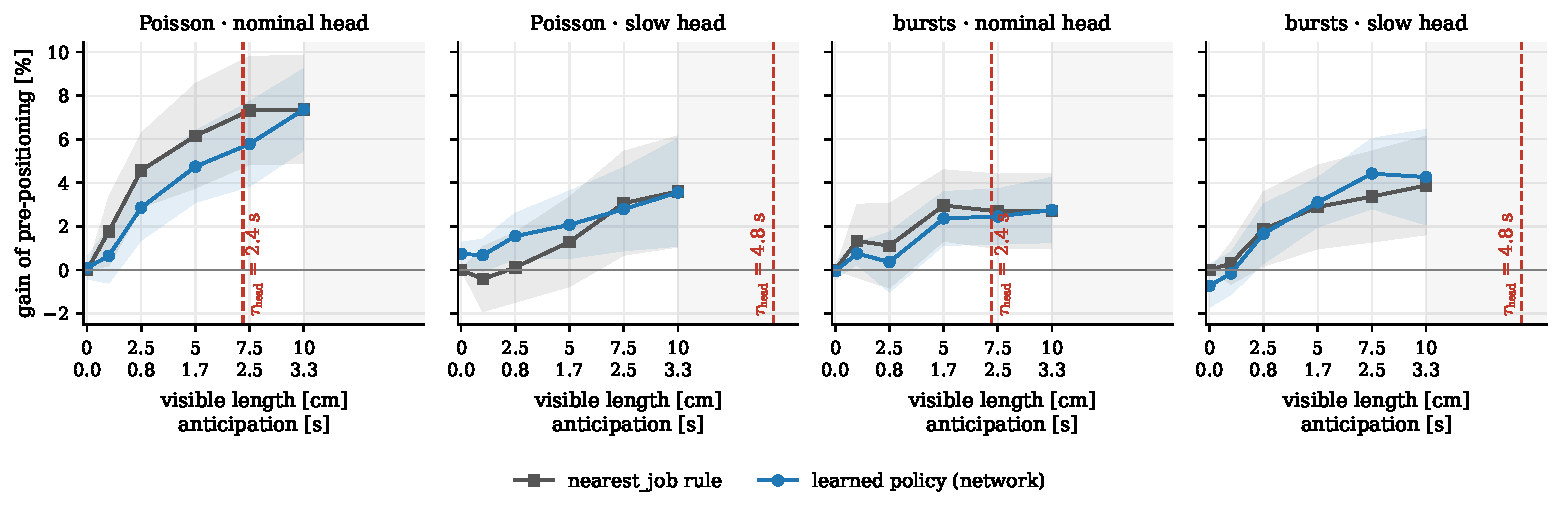
\includegraphics[width=\linewidth]{figures/coverage_real.pdf}
\caption{Reference cell, nominal load: reduction of the penalized flow time obtained by
pre-positioning (\texttt{when\_idle} against \texttt{none} at the same visible length,
paired; bands are 95\,\% CIs) against the visible length and the anticipation
$\tv=\lv/\vb$. The dashed line is the head's travel time across the conveyors,
$\tcross$; the shaded area lies beyond the entry zone. Seeds 7000--7029, shared with the companion paper.}
\label{fig:coverage}
\end{figure}

The share answers how much of the benefit a shorter view retains; the designer's question
is how much worse the cell is, already pre-positioning, with a shorter view
(Table~\ref{tab:direct}): at the nominal regime, 7.5~cm instead of 10~cm costs
$+0.24\pm0.57$\,\% for the network and $+0.05\pm0.04$\,\% for the rule, against
$+1.33\pm0.91$ and $+1.36\pm0.86$\,\% with 5~cm; with the slow head 7.5~cm costs
$1.4\pm1.1$ and $0.7\pm1.8$\,\%, and 5~cm $2.2\pm1.5$ and $2.7\pm2.3$\,\%. The two readings
differ for the network because its \texttt{none} level at 7.5~cm is $1.4\pm1.0$ points
below its level at 10~cm, which the share counts as benefit lost and the direct contrast
does not carry. Read against $\tcross$, this curve suggested that the head's crossing time
is the reference for sizing the coverage; that reading, formed on one geometry, is the
hypothesis the geometry bench was built to test.

\begin{table}[t]
\centering\small
\caption{Reference cell: two answers to ``is a shorter view enough?'' Left: cost of
pre-positioning with 5 or 7.5~cm against with the whole 10~cm zone (\texttt{when\_idle}
at both lengths; paired $\Delta$ of the penalized flow time, \%, 95\,\% CI; positive = the
shorter view costs more; in parentheses, realizations in which the shorter view was
better). Right: pre-positioning benefit lost, the gain of Supplementary
Table~\ref{S-tab:coverage} at the shorter length minus the gain at 10~cm, per realization
(points). A secondary analysis of the phase-4 data, added after the run. Bold: the
interval excludes zero. Seeds 7000--7029, shared with the companion paper.}
\label{tab:direct}
\resizebox{\linewidth}{!}{% generated by experiments/paper2_figures.py from data/phase4_info.csv
\begin{tabular}{@{}llcccc@{}}
\toprule
regime & policy & \multicolumn{2}{c}{5 cm against 10 cm} & \multicolumn{2}{c}{7.5 cm against 10 cm} \\
 & & cost [\%] & benefit lost [pts] & cost [\%] & benefit lost [pts] \\
\midrule
real / Poisson / nominal head & \textsc{nj} & {\boldmath$+1.36 \pm 0.86$} (2/30) & {\boldmath$+1.21 \pm 0.78$} & {\boldmath$+0.05 \pm 0.04$} (0/30) & {\boldmath$+0.05 \pm 0.04$} \\
 & network & {\boldmath$+1.33 \pm 0.91$} (5/30) & {\boldmath$+2.63 \pm 1.04$} & $+0.24 \pm 0.57$ (5/30) & {\boldmath$+1.59 \pm 1.08$} \\
real / Poisson / slow head & \textsc{nj} & {\boldmath$+2.70 \pm 2.32$} (8/30) & {\boldmath$+2.32 \pm 2.19$} & $+0.73 \pm 1.82$ (6/30) & $+0.55 \pm 1.78$ \\
 & network & {\boldmath$+2.23 \pm 1.46$} (5/30) & $+1.48 \pm 1.88$ & {\boldmath$+1.36 \pm 1.11$} (3/30) & $+0.77 \pm 1.51$ \\
real / bursts / nominal head & \textsc{nj} & $-0.22 \pm 0.67$ (4/30) & $-0.24 \pm 0.70$ & $+0.03 \pm 0.04$ (0/30) & $+0.03 \pm 0.04$ \\
 & network & $+0.34 \pm 0.55$ (5/30) & $+0.39 \pm 0.94$ & $+0.29 \pm 0.42$ (1/30) & $+0.30 \pm 0.94$ \\
real / bursts / slow head & \textsc{nj} & $+1.21 \pm 1.72$ (7/30) & $+0.99 \pm 1.64$ & $+0.59 \pm 0.80$ (2/30) & $+0.51 \pm 0.74$ \\
 & network & $+1.60 \pm 1.97$ (6/30) & $+1.16 \pm 1.85$ & $+0.19 \pm 1.48$ (6/30) & $-0.16 \pm 1.56$ \\
\midrule
heavy / Poisson / nominal head & \textsc{nj} & $+0.24 \pm 0.84$ (6/30) & $+0.22 \pm 0.82$ & $+0.43 \pm 0.93$ (4/30) & $+0.40 \pm 0.92$ \\
 & network & $+0.29 \pm 0.96$ (9/30) & $+0.50 \pm 1.25$ & $-0.60 \pm 1.09$ (9/30) & $-0.21 \pm 1.32$ \\
heavy / Poisson / slow head & \textsc{nj} & $+0.29 \pm 1.82$ (16/30) & $+0.19 \pm 1.83$ & $+0.35 \pm 1.52$ (17/30) & $+0.24 \pm 1.46$ \\
 & network & $+0.50 \pm 1.98$ (16/30) & $+0.71 \pm 2.25$ & $+0.11 \pm 1.51$ (19/30) & $+0.17 \pm 1.54$ \\
heavy / bursts / nominal head & \textsc{nj} & $-0.24 \pm 1.24$ (12/30) & $-0.31 \pm 1.24$ & $+0.24 \pm 0.70$ (7/30) & $+0.22 \pm 0.71$ \\
 & network & $+0.83 \pm 0.95$ (6/30) & {\boldmath$+1.01 \pm 0.92$} & $+0.03 \pm 0.59$ (9/30) & $-0.05 \pm 0.69$ \\
heavy / bursts / slow head & \textsc{nj} & $+1.29 \pm 1.75$ (12/30) & $+1.16 \pm 1.90$ & $+0.93 \pm 1.55$ (13/30) & $+0.83 \pm 1.65$ \\
 & network & $+0.78 \pm 1.45$ (11/30) & $+0.52 \pm 1.30$ & $+0.42 \pm 1.16$ (12/30) & $+0.51 \pm 1.10$ \\
\bottomrule
\end{tabular}
}
\end{table}

%====================================================================
\section{The geometry bench at 3~cm/s}\label{sec:benchresults}
%====================================================================

\subsection{Where pre-positioning pays}\label{sec:worth}
Table~\ref{tab:gains} gives the whole-grid gain $G(10\,\mathrm{s})$ of the rule
(arrival-time tie-break, seeds 9000--9059) in the 56 distinct cells. It spans $-0.08$ to
$+2.44$~s per part, and passes the frozen benefit criterion in \textbf{18 cells}: 13 with
Poisson arrivals and 5 with bursts; 10 of the 28 nominal-load and 8 of the 28 high-load
cells; 10 of the 28 cells with $v_x=5$~cm/s and 8 of the 28 with $v_x=10$. At the nominal
load the gain with bursts is about half of the gain with Poisson arrivals in the
corresponding geometries (0.4--1.5 against 0.8--2.4~s per part). At the high load the
gains are $-0.1$ to $2.0$~s per part with half-widths of 0.5--1.6~s, so most undetermined
cells there are undetermined by precision rather than by size; at the nominal load with
bursts they are undetermined by size. The gain is 82--96\,\% unpenalized flow time. The
rule's coverage curves for every cell are in \supsec{sup:curves}. The network, run as
secondary controller, passes the benefit criterion in 17 of the 72 regimes and reaches no
conservative knee before 10~s (\supsec{sup:benchnet}).

\begin{table}[t]
\centering\small
\caption{Geometry bench, \nj\ (arrival-time tie-break, seeds 9000--9059): gain of
pre-positioning with the whole grid,
$G(10\,\mathrm{s})=J_{\mathrm{none}}-J_{\mathrm{when\_idle}}$ at 10~s of anticipation
[s per part], paired over 60 realizations, 95\,\% CI. Columns: the seven distinct
crossing times with the geometry that realizes them (cells with the same $\tcross$ are
identical, \supsec{sup:checks}). Bold: worth sizing the coverage for ($G\ge1$~s per part,
lower bound $\ge0.5$).}
\label{tab:gains}
\resizebox{\linewidth}{!}{% generated by experiments/paper2_bench_figures.py from data/geometry_bench.csv.gz
\begin{tabular}{@{}lllccccccc@{}}
\toprule
$v_x$ & load & arrivals & $\tau_{\mathrm{cross}}=0.8$~s & $\tau_{\mathrm{cross}}=1.2$~s & $\tau_{\mathrm{cross}}=1.6$~s & $\tau_{\mathrm{cross}}=2.4$~s & $\tau_{\mathrm{cross}}=3.6$~s & $\tau_{\mathrm{cross}}=4.8$~s & $\tau_{\mathrm{cross}}=7.2$~s \\
 & & & 6~cm / 15~cm/s & 6~cm / 10~cm/s & 12~cm / 15~cm/s & 12~cm / 10~cm/s & 18~cm / 10~cm/s & 12~cm / 5~cm/s & 18~cm / 5~cm/s \\
\midrule
5 & nominal & Poisson & {\boldmath$+2.44 \pm 0.78$} & {\boldmath$+2.35 \pm 0.88$} & {\boldmath$+1.49 \pm 0.67$} & {\boldmath$+2.05 \pm 0.73$} & $+1.18 \pm 0.91$ & $+0.99 \pm 1.07$ & $+1.14 \pm 1.19$ \\
5 & nominal & bursts & $+1.05 \pm 0.62$ & $+1.21 \pm 0.76$ & {\boldmath$+1.04 \pm 0.46$} & $+0.98 \pm 0.74$ & $+0.88 \pm 0.74$ & $+0.94 \pm 0.93$ & {\boldmath$+1.50 \pm 0.95$} \\
5 & high & Poisson & $+1.30 \pm 1.07$ & $+1.51 \pm 1.08$ & $+1.00 \pm 1.18$ & $+1.52 \pm 1.15$ & {\boldmath$+1.73 \pm 1.04$} & {\boldmath$+2.02 \pm 1.47$} & $+0.10 \pm 1.64$ \\
5 & high & bursts & $+1.27 \pm 0.95$ & {\boldmath$+1.49 \pm 0.87$} & $+1.07 \pm 0.74$ & $+0.97 \pm 1.02$ & {\boldmath$+1.97 \pm 0.98$} & $+1.05 \pm 0.77$ & $+0.10 \pm 0.85$ \\
\midrule
10 & nominal & Poisson & {\boldmath$+1.03 \pm 0.26$} & {\boldmath$+1.19 \pm 0.35$} & {\boldmath$+1.26 \pm 0.31$} & {\boldmath$+1.32 \pm 0.38$} & $+0.78 \pm 0.45$ & $+0.88 \pm 0.60$ & $+0.80 \pm 0.70$ \\
10 & nominal & bursts & $+0.43 \pm 0.29$ & $+0.51 \pm 0.30$ & $+0.46 \pm 0.30$ & $+0.60 \pm 0.28$ & $+0.59 \pm 0.39$ & $+0.96 \pm 0.54$ & $+0.95 \pm 0.52$ \\
10 & high & Poisson & {\boldmath$+1.26 \pm 0.56$} & {\boldmath$+1.25 \pm 0.50$} & {\boldmath$+1.19 \pm 0.59$} & $+0.87 \pm 0.64$ & $+0.83 \pm 0.84$ & $+0.98 \pm 0.70$ & $+0.49 \pm 0.71$ \\
10 & high & bursts & {\boldmath$+1.03 \pm 0.51$} & $+0.38 \pm 0.58$ & $+0.44 \pm 0.57$ & $+0.45 \pm 0.51$ & $+0.92 \pm 0.52$ & $+0.55 \pm 0.58$ & $-0.08 \pm 0.48$ \\
\bottomrule
\end{tabular}
}
\end{table}

\subsection{The cost of a shorter view in three analyses}\label{sec:cost}\label{sec:tiebreak}
The bench ran the rule with its legacy tie-break, the arrival time, which may precede the
first observation of a part; those results were fixed before the run. After the run, as a
retrospective sensitivity analysis and not as a new confirmation, the rule was rerun on the
same 60 realizations with the observable tie-break (the instant of first observation) and
the criteria unchanged; under that key the pure-information contrast of the rule is no
longer zero by construction, so $G$ at each coverage is measured against a baseline that
can move with it. The observable-key result was then replicated on 60 fresh realizations
(seeds 43700--43759), with everything fixed before the run. Each analysis applies the
benefit screen independently (Table~\ref{tab:cohorts}; per-cell results in
\supsec{sup:cohorts}).

\begin{table}[t]
\centering\small
\caption{The three analyses of the 3~cm/s geometry bench with \nj: the prespecified run
(arrival-time tie-break), its retrospective rerun with the observable tie-break on the
same realizations, and the replication with the observable tie-break on fresh
realizations. Each analysis applies the benefit screen independently; knees and costs as
in Supplementary Table~\ref{S-tab:sufficient}; the cost interval is the individual paired
95\,\% interval of the cell with the largest estimated cost.}
\label{tab:cohorts}
\resizebox{\linewidth}{!}{%
\begin{tabular}{@{}lccccc@{}}
\toprule
analysis & pass the screen & knee $<10$~s & cons.\ knee $<10$~s & cost of 3.33~s, median & largest [95\,\% CI] \\
\midrule
arrival-time key, seeds 9000--9059 & 18/56 & 18/18 & 17/18 & 0.05 & 0.44 [0.11, 0.77] \\
observable key, seeds 9000--9059 & 19/56 & 17/19 & 3/19 & 0.04 & 0.44 [$-0.01$, 0.89] \\
observable key, seeds 43700--43759 & 14/56 & 13/14 & 1/14 & 0.09 & 0.47 [0.02, 0.91] \\
\bottomrule
\end{tabular}}
\end{table}

\textbf{Arrival-time key, seeds 9000--9059 (18 cells).} Giving the controller 3.33~s of
anticipation (10~cm of belt at 3~cm/s, the reference cell's entry zone) instead of 10~s
cost a median of 0.05~s per part and at most 0.44~s per part, the largest estimate among
the 18 cells (individual 95\,\% interval 0.11--0.77), not an upper bound for the family;
the cost is significant in 5 of the 18. In share terms, 3.33~s retained 71--102\,\% of the
whole-grid gain (median 97\,\%).

\textbf{Observable key, same seeds (19 cells).} The benefit criterion passes 19 cells
instead of 18; 13 pass under both keys, 5 only under the arrival-time key and 6 only under
the observable one. In the 19 cells, 3.33~s instead of 10~s cost a median of 0.04~s per
part and at most 0.44~s, the largest estimate among the 19 cells and not an upper bound for
the family (individual 95\,\% interval $-0.01$ to 0.89; the maxima of the two keys come from
different cells); no
interval excludes zero on the side of a loss, and one excludes it on the other side
($d/v_y/v_x=12/15/5$, high load, bursts: the shorter view was cheaper by $0.54\pm0.39$~s per
part). The share retained at 3.33~s was 58--130\,\%.

\textbf{Observable key, fresh seeds 43700--43759 (14 cells).} Fourteen cells pass; 9 of them
also passed with the observable key on the original realizations, 10 with the
arrival-time key, and 8 in all three analyses. Giving the controller 3.33~s instead of 10~s
cost a median of 0.09 and at most 0.47~s per part, the largest estimate among the 14 cells
($18/5/5$, nominal load, bursts; individual 95\,\% interval 0.02--0.91), not an upper bound
for the family, with an interval excluding zero in 2 of the 14 cells and an upper limit at
or below 0.5~s per part in 9; the share retained at 3.33~s was 67--117\,\%. The intervals
are per cell, computed after the screen and without adjustment for choosing the largest
estimate.

In all three analyses a view of 3.33~s cost little on average in the cells where
pre-positioning pays, though not in every cell, and which cells pass the benefit screen is
not stable across realizations. The cost and the share answer different design questions:
the direct cost is what the cell loses by seeing less; the retention is whether a fixed
fraction of the benefit can be guaranteed.

\subsection{Certifying 90\,\% retention}\label{sec:retention}
With the arrival-time key the knee that retains 90\,\% of the gain lies at 0.5--5~s as a
point estimate (median 2.5~s over the 18 cells: 1.75~s at $v_x=10$ and 3.33~s at
$v_x=5$~cm/s) and at 2.0--7.5~s conservatively, with one cell undetermined ($d=12$,
$v_y=5$, $v_x=5$, high load, Poisson, where no grid point is conservatively at 90\,\%). The
two answers differ because the curves are flat near their top: a cell can retain 95\,\% of
its gain at 3.33~s and still need 5--7.5~s before the paired contrast against 90\,\% of the
top is conservatively positive. The protocol fixed the conservative result as the
headline of the bench: 17 of the 18 cells reached the 90\,\% criterion with 2.0--7.5~s.

With the observable key on the same realizations the conservative criterion is first met
before 10~s in 3 of the 19 cells (at 2, 7.5 and 7.5~s) and first at 10~s, the end of the
grid, in the other 16. Of the 13 cells that pass under both keys, all 13 certify before
10~s under the arrival-time key and 3 under the observable key. On fresh realizations the
point estimate first reaches 90\,\% before 10~s in 13 of the 14 cells, the conservative
criterion in 1 ($6/15/10$, nominal load, Poisson arrivals, at 2~s). The change is not only
one of precision: the set of cells, the estimated curves and their uncertainty all change,
and in two cells of the rerun ($18/10/5$ at the high load with bursts and at the nominal
load with Poisson arrivals) even the point estimate first reaches 90\,\% only at 10~s. A
fixed heuristic need not respond monotonically to a wider view, and under the observable
key its baseline moves with the coverage. A first certification at the last grid point
describes the uncertainty and the coverages tested in that cell; it does not show that
10~s of coverage is physically required. Early certification of 90\,\% retention is thus a
property of the arrival-time key.

\subsection{The along-belt axis is a first-order factor}\label{sec:vx}\label{sec:predict}
At the nominal load with Poisson arrivals (arrival-time key), halving $v_x$ from 10 to
5~cm/s multiplied the gain of pre-positioning by 1.2--2.4 in the four geometries
($\tcross\le2.4$~s) in which both speeds pass the benefit criterion (1.03--1.32 $\to$
1.49--2.44~s per part; by 1.1--1.5 in the three geometries in which neither does),
lengthened the mean along-belt component of the moves from 0.44--0.76 to 1.57--1.90~s in
those four cells, lowered the head's idle fraction under \texttt{none} from 17--27\,\% to
12--15\,\%, and moved the knee from 1.5--3.33~s (conservatively 2.0--3.33) to 3.33--5~s
(conservatively 5--7.5). The size of the change depends on the geometry; its direction does
not. In these runs the anticipation the camera must give was associated with the whole
move, and the along-belt part of it does not scale with the belt spacing.

\textbf{Predictors.} Among the predictors of the point-estimate knee fixed before the run
(18 cells, arrival-time key), the crossing-time family is the poorest (leave-one-out mean
absolute error 1.53~s unscaled, 1.75~s rescaled), since it ignores the along-belt part of
the moves; the mean planned duration of the pre-positioning moves, $\tpp$, is the best
(1.02~s, fitted knee $\approx1.74\,\tpp$), a constant of 2.76~s close behind (1.13~s), and a
group mean by $v_x$ computed after the run does better than both (0.82~s); on the 19 cells
of the observable key (seeds 9000--9059) the move duration and that group mean are within
0.03~s of each other (1.72 and 1.74~s). The errors are two to three steps of the fine end
of the grid, and $\tpp$ needs full-view traces. None of the predictors probed supports
extrapolation to cells that differ much from those tested: the data support a number of
seconds of anticipation for this family of cells at 3~cm/s, not a predictor
(\supsec{sup:predict}).

\textbf{Further analyses.} The traces are compatible, at the nominal load, with the saving
of a pre-positioning move being transmitted to the parts queued behind it; at the high
load the queue count does not explain the size of the effect (\supsec{sup:mechanism}).
Lengthening the physical entry zone from 10 to 35~cm in the reference geometry adds
10.35--13.19~s per part to the rule's $J$, while no difference in the gain of
pre-positioning at a given anticipation was detected (\supsec{sup:entry}).

%====================================================================
\section{The belt-speed bench: what transfers to 5~cm/s}\label{sec:belt}
%====================================================================
Table~\ref{tab:belt} gives the belt-speed bench of Section~\ref{sec:beltdesign} (11\,520
episodes; no candidate upstream of the visible stretch, identical arrivals at both speeds
in all 240 cell--realization pairs). Its check column reproduces the 3~cm/s costs of the
geometry bench with the 50~cm entry: $C_3(10\,\mathrm{cm})$ is $+0.10\pm0.47$,
$+0.18\pm0.23$, $-0.15\pm0.26$ and $-0.11\pm0.17$~s per part in the four cells, every
interval containing the value of the geometry bench.

\begin{table}[t]
\centering\small
\caption{Belt-speed bench, \nj\ with the observable tie-break, nominal load, Poisson
arrivals, 50~cm entry, 60 paired realizations (seeds 10000--10059, used once): the full-view benefit
$G_v(50\,\mathrm{cm})$ at 3 and at 5~cm/s with the benefit criterion, the paired costs at
5~cm/s of 10~cm (2.00~s) and 16.7~cm (3.33~s) against 50~cm, the check column
$C_3(10\,\mathrm{cm})$ (the 3.33~s cost at 3~cm/s, to be compared with
Section~\ref{sec:cost}), and the frozen verdict (conservative reading, margin 0.5~s per
part). Seconds per part, 95\,\% CI.}
\label{tab:belt}
\resizebox{\linewidth}{!}{% generated by experiments/paper2_bench_figures.py from data/belt_speed_bench.csv.gz
\begin{tabular}{@{}lcccccccl@{}}
\toprule
cell & $G_3(50\,\mathrm{cm})$ & useful at 3 & $G_5(50\,\mathrm{cm})$ & useful at 5 & $C_5(10\,\mathrm{cm})$ & $C_5(16.7\,\mathrm{cm})$ & $C_3(10\,\mathrm{cm})$ & verdict at 5~cm/s \\
 & [s/part] & & [s/part] & & $=2.00$~s & $=3.33$~s & $=3.33$~s (check) & (conservative) \\
\midrule
$d=12$, $v_y=10$, $v_x=5$ ($\tcross=2.4$~s) & $+1.74 \pm 0.87$ & yes & $+0.62 \pm 0.73$ & no & $-0.00 \pm 0.51$ & $+0.12 \pm 0.39$ & $+0.10 \pm 0.47$ & full-view benefit criterion not met at 5~cm/s \\
$d=12$, $v_y=10$, $v_x=10$ ($\tcross=2.4$~s) & $+0.99 \pm 0.38$ & no & $+1.76 \pm 0.39$ & yes & $+0.06 \pm 0.26$ & $-0.02 \pm 0.24$ & $+0.18 \pm 0.23$ & 10~cm keep the benefit ($H_{\mathrm{cm}}$) \\
$d=6$, $v_y=15$, $v_x=5$ ($\tcross=0.8$~s) & $+1.58 \pm 0.89$ & yes & $+0.47 \pm 0.55$ & no & $+0.48 \pm 0.55$ & $+0.12 \pm 0.45$ & $-0.15 \pm 0.26$ & full-view benefit criterion not met at 5~cm/s \\
$d=6$, $v_y=15$, $v_x=10$ ($\tcross=0.8$~s) & $+1.16 \pm 0.34$ & yes & $+1.22 \pm 0.37$ & yes & $+0.05 \pm 0.18$ & $+0.00 \pm 0.14$ & $-0.11 \pm 0.17$ & 10~cm keep the benefit ($H_{\mathrm{cm}}$) \\
\bottomrule
\end{tabular}
}
\end{table}

\textbf{At 5~cm/s, 10~cm of coverage cost less than the margin in the two cells with
$v_x=10$~cm/s}: the upper 95\,\% bounds of $C_5(10\,\mathrm{cm})$ are 0.33 and 0.23~s per
part, below the margin of 0.5 ($H_{\mathrm{cm}}$, conservative), and no difference
between 16.7 and 10~cm was detected there (direct paired contrast 10 minus 16.7~cm:
$+0.09\pm0.26$ and $+0.05\pm0.14$~s per part). The 90\,\% retention criterion, however,
is not certified at 10~cm in either fast cell at 5~cm/s: the first conservatively
certified length is 25~cm in $d=12$, $v_y=10$, $v_x=10$ and 50~cm in $d=6$, $v_y=15$,
$v_x=10$; the margin and the certification are different questions. As written
beforehand, these two cells cannot separate the two scales, so their result is the
practical one, 10~cm suffice at 5~cm/s, not a mechanistic one. One premise check: with the
50~cm entry, the cell $d=12$, $v_y=10$, $v_x=10$ sits on the benefit threshold at 3~cm/s
($+0.99\pm0.38$ against the criterion's 1.0, lower bound 0.61 against 0.5), so it does not
pass the benefit criterion at 3~cm/s in this bench; it is reported as it falls.

\textbf{At 5~cm/s, neither of the two slow-axis cells met the benefit criterion with
the full view; the paired comparison between speeds detected a reduction in one of the
two.} $G_5(50\,\mathrm{cm})=+0.62\pm0.73$ and $+0.47\pm0.55$~s per part, against
$+1.74\pm0.87$ and $+1.58\pm0.89$ at 3~cm/s; paired across speeds, 3 minus 5~cm/s, the
difference is $+1.12\pm1.21$ in $d=12$, $v_y=10$, $v_x=5$ (not detected) and
$+1.11\pm1.02$ in $d=6$, $v_y=15$, $v_x=5$ (detected). The frozen verdict (``benefit lost at
this speed'' in the protocol, ``full-view benefit criterion not met at 5~cm/s'' in
Table~\ref{tab:belt}) follows from the precedence of the benefit criterion, so the coverage
question is moot there; on the shorter views themselves the conservative reading is
undetermined: $C_5(16.7\,\mathrm{cm})=+0.12\pm0.39$ and $+0.12\pm0.45$~s per part have upper
bounds of 0.51 and 0.57, above the margin, so $H_{\mathrm{neither}}$ is neither established
nor excluded. In the fast-axis cells the full-view benefit rose at the faster belt in
$d=12$, $v_y=10$, $v_x=10$ ($-0.77\pm0.60$, 3 minus 5~cm/s) and no difference was detected
in $d=6$, $v_y=15$, $v_x=10$ ($-0.06\pm0.53$).

\textbf{The comparison between centimetres and seconds remains open}: the cells that
could have separated the two readings are the ones that lost the benefit, and the
descriptive alignment reading fixed beforehand favours the time scale in three cells and
the distance scale in one, with a post hoc caveat that the matched-anticipation pairs sit
where both curves are flatter. The coverage curves, the traces and the effect of the
observable tie-break on the \texttt{none} level are in \supsec{sup:belt}.

%====================================================================
\section{Discussion}\label{sec:discussion}
%====================================================================

\textbf{A specification in seconds, with a practical extension to 5~cm/s.} At 3~cm/s the
direct cost of a shorter view was small on average in all three analyses, though not in
every cell, and the largest observed costs are estimates with individual intervals
reaching 0.77--0.91~s per part, not bounds for the family; the conservative 90\,\%
requirement (2--5~s at $v_x=10$~cm/s and 5--7.5~s at $v_x=5$~cm/s with the arrival-time
key) is not supported by the observable key. Within the geometry bench seconds of belt
motion and centimetres are one unit; the clock time a camera gives is longer whenever the
belt stops. The physical argument for seconds is that the anticipation must cover the
head's move, which does not depend on $\vb$; but changing $\vb$ also changes where the head
intercepts each part. The belt-speed bench gives the practical answer for 5~cm/s without
settling the scale (\supsec{sup:discussion}).

\textbf{Why widening the view alone changes little.} Under treatment~B the controller must
choose among the parts already in the zone whenever there is one; upstream visibility can
help it only through the order of the zone parts. For the rule with the arrival-time
tie-break this help is zero by construction; an average near zero for the network measures
what this policy extracts from the view, not what an optimal policy could. The exception is
the high load with bursts, where the network gains up to 1.6~s per part from the view alone
in the geometry bench, the regime in which the reference study also found its one
significant B-vs-A cell.

\textbf{Load, bursts and idle time.} Pre-positioning is an action for an idle head. The
number of opportunities is limited by the head's idle time, which falls with the load and
with slower heads, and bursts spend the opportunities on the first part of each burst. This is one
possible reason why the cells worth sizing for are concentrated at Poisson arrivals and why the
high-load cells are mostly undetermined by precision.

\subsection{Limits}\label{sec:limits}
What these results do not establish:
\begin{itemize}[nosep]
\item \emph{A minimum physical length}: a first certification at the end of the grid does
  not show that 10~s of coverage is physically required, and the designs are a predefined
  grid compared on paired realizations, not optimized jointly with the controller as line
  parameters are in \cite{Sarker2001}.
\item \emph{A scale law between seconds and centimetres}: the belt-speed bench covers four
  cells at the nominal load with Poisson arrivals and the rule alone, and the cells that
  could separate the scales lost the benefit at 5~cm/s; a bench that keeps a useful benefit
  at both speeds in cells with a slow along-belt axis (a lower load, or a longer laser zone)
  would settle it.
\item \emph{Cells outside the family}: three belts, a 35~cm laser zone, constant processing
  of 2.5~s, two loads; 38 of the 56 cells are undetermined, some by size and some by
  precision; parts are points with a minimum spacing, the head has no acceleration, and the
  network is a secondary controller whose training ranges the bench partly exceeds.
\item \emph{An economic value}: the penalty weights are placeholders, and the benefit
  screen is sensitive to them (15 instead of 18 cells on the raw flow time); the study
  measures the camera's reach, not its precision, latency or losses.
\item \emph{A causal propagation of the saving to the queue}: the reading of the gain per
  move as a saving passed on to the parts queued behind it is a compatibility argument.
\end{itemize}
The rule's tie-break differs between studies (arrival time in the first two, observable
instant in the third). The three sets of reserved realizations were used once for their
prespecified analyses; those of the geometry bench were reused for the retrospective
rerun, and the replication used a fourth, fresh set.

%====================================================================
\section{Conclusions}
%====================================================================
At a belt speed of 5~cm/s, with the rule and its observable tie-break, a 10~cm view cost
less than the margin of 0.5~s per part fixed beforehand against the full 50~cm view in the
two tested geometries with the fast along-belt head axis, while neither slow-axis geometry
met the full-view benefit criterion, and the comparison between centimetres and seconds
remains open. In the reference cell, the value of the camera was mostly the value of the
action it enables: allowing the idle head to move towards a visible part reduced the
penalized flow time by 7.4\,\% at the nominal load for both controllers (2.7--4.3\,\% with
bursts or a slow head), while widening the view alone produced small effects. At 3~cm/s, in
the cells where pre-positioning pays, 3.33~s of anticipation instead of 10~s cost a median
of 0.05, 0.04 and 0.09~s per part in the three analyses (the rule with the arrival-time and
the observable tie-break on seeds 9000--9059, and with the observable tie-break on fresh
seeds 43700--43759), with largest observed estimates of
0.44, 0.44 and 0.47~s per part. Certified 90\,\% retention before 10~s (17 of 18 cells) is
a property of the arrival-time tie-break (3 of 19 on the same realizations and 1 of 14 on
fresh ones with the observable tie-break), and
which cells pass the benefit screen is not stable across realizations. The along-belt head
speed is a first-order factor, and for this family of cells at 3~cm/s the camera is best
specified in seconds of anticipation, with the cost of a shorter view measured, not by a
predictor to extrapolate.

\bibliographystyle{plain}
\bibliography{../../literature/references}

\end{document}
